\documentclass[10pt,a4paper]{article}

\usepackage{amsmath}
\usepackage{graphicx}
\usepackage{float}
\usepackage[polish]{babel}
\usepackage[utf8]{inputenc}
\usepackage{polski}
\frenchspacing


\author{Marcin Ochman}
\title{Tablice mieszające}

\begin{document}
\maketitle
\section{Opis problemu}

Tablice asocjacyjne to wygodna struktura danych, która pozwala dostać się do danych przy użyciu
klucza. Istnieje kilka różnych pomysłów, jak taką strukturę zaimplementować.U mnie można znaleźć
trzy różne rozwiązania:
\begin{itemize}
\item tablica mieszająca z dowiązaniem łańcuchowym
\item użycie \textit{std::vector}, klucze są dodawane tak, że są zawsze posortowane
\item użycie drzewa przeszukiwań binarnych
\end{itemize}

Każde z tych rozwiązań ma swoje wady i zalety, jednak \underline{średni} czas znalezienia wartości
przechowywanej pod podanym kluczem wynosi $\mathcal{O}(lg(n))$ (przy braku kolizji w tablicy
mieszającej, drzewo binarne bliskie zrównoważenia).


\section{Sposób implementacji funkcji mieszającej dla łańcuchów znaków}

Funkcja mieszająca zaimplementowana jest w bardzo prosty ale sprawdzony sposób.
Każdy kod litery jest mnożony przez wagę, która jest odpowiednim indeksem litery w łańcuchu
powiększonym o jeden. Wszystko jest sumowane, a następnie brana jest tylko reszta z dzielenia przez 10000.

\section{Wyniki przeprowadzonych testów}

Test polegał na zmierzeniu czasu dostępu do wartości, która została dodana na samym końcu.
Ze względu na to, że implementacja na \textit{std::vector} dodaje element w czasie
liniowym, trwa to bardzo długo, dlatego ograniczyłem się w tym przypadku do 150000
elementów. Dla pozostałych tablic maksymalny rozmiar to 1,5 miliona elementów. Wyniki testów są
przedstawione na poniższych wykresach

\begin{figure}[H]
\centering
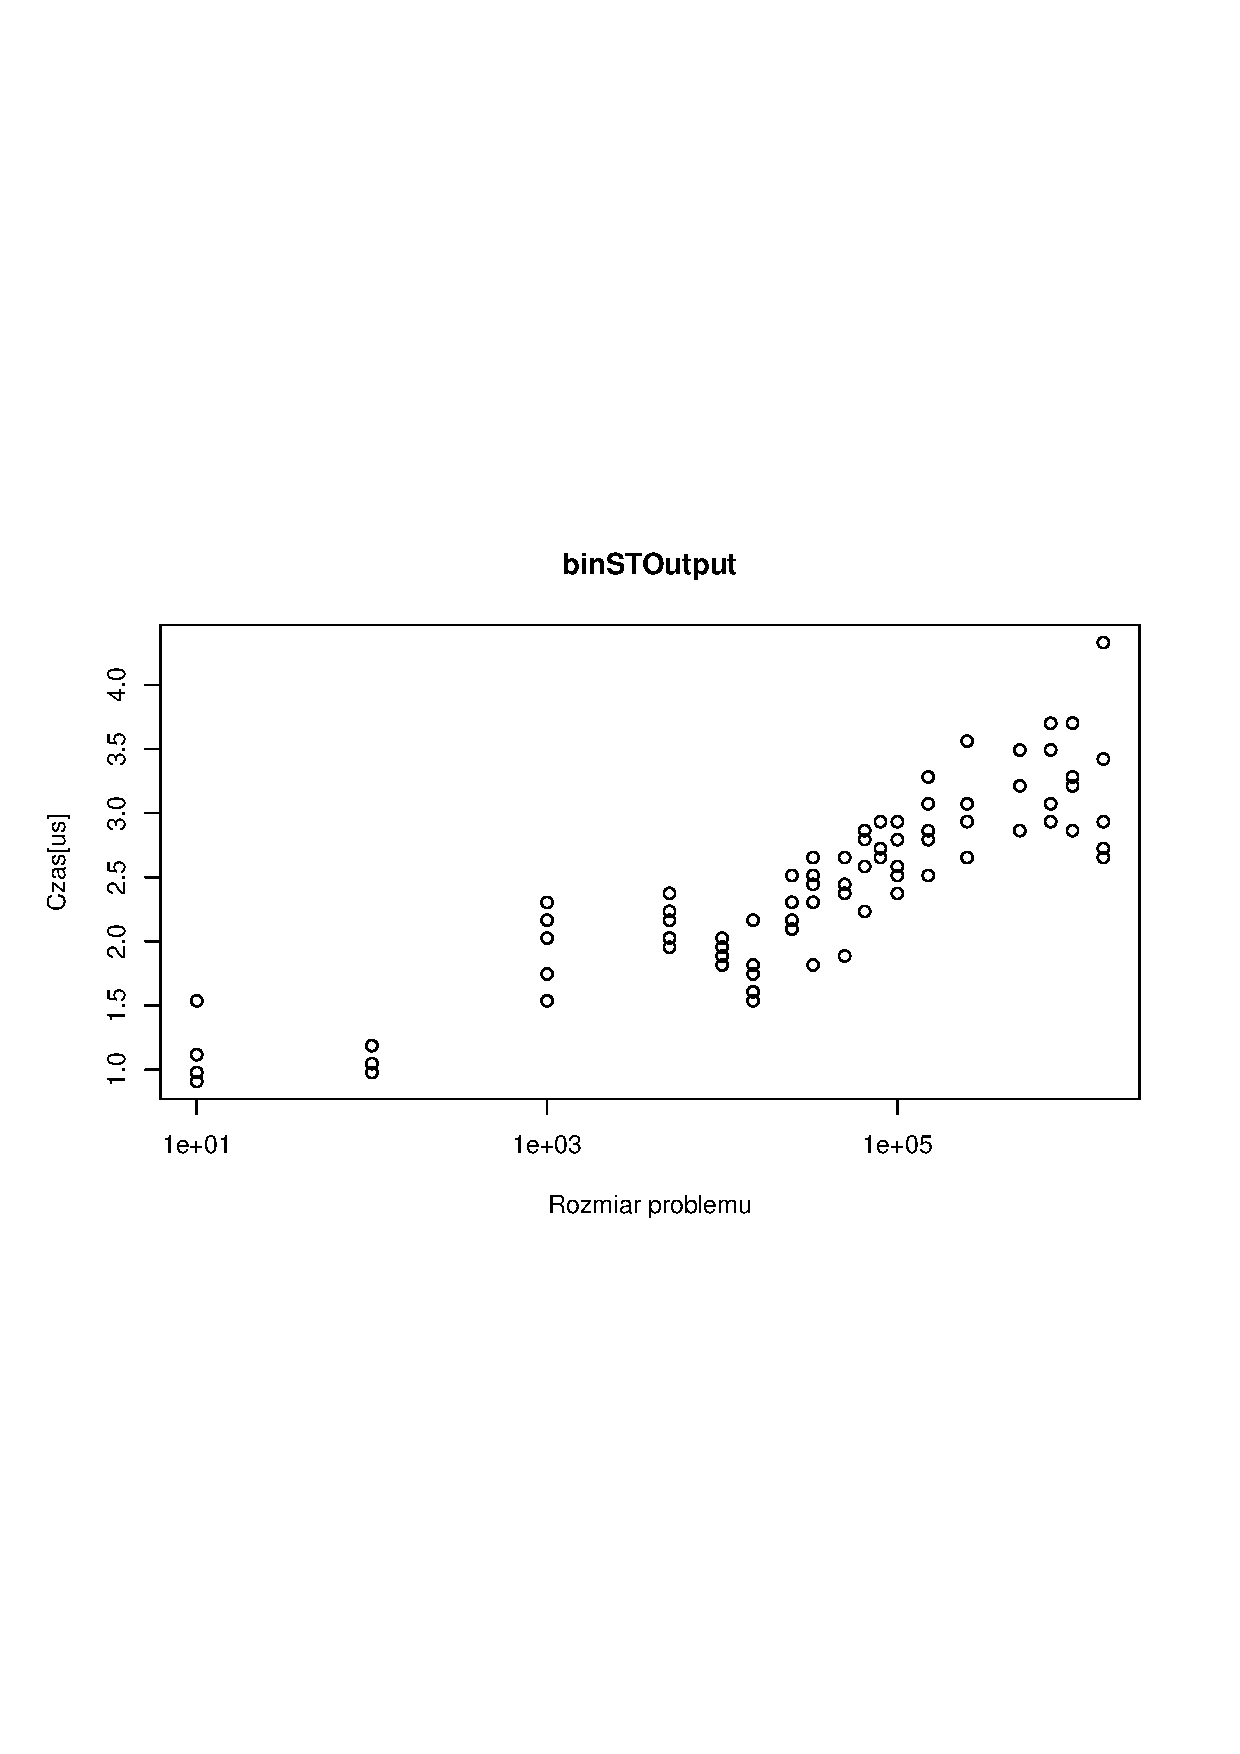
\includegraphics[width=0.7\linewidth]{./Wykresy/binSTOutput}
\caption{Wyniki dla drzewa przeszukiwań binarnych}
\label{fig:binSTOutput}
\end{figure}


\begin{figure}[H]
\centering
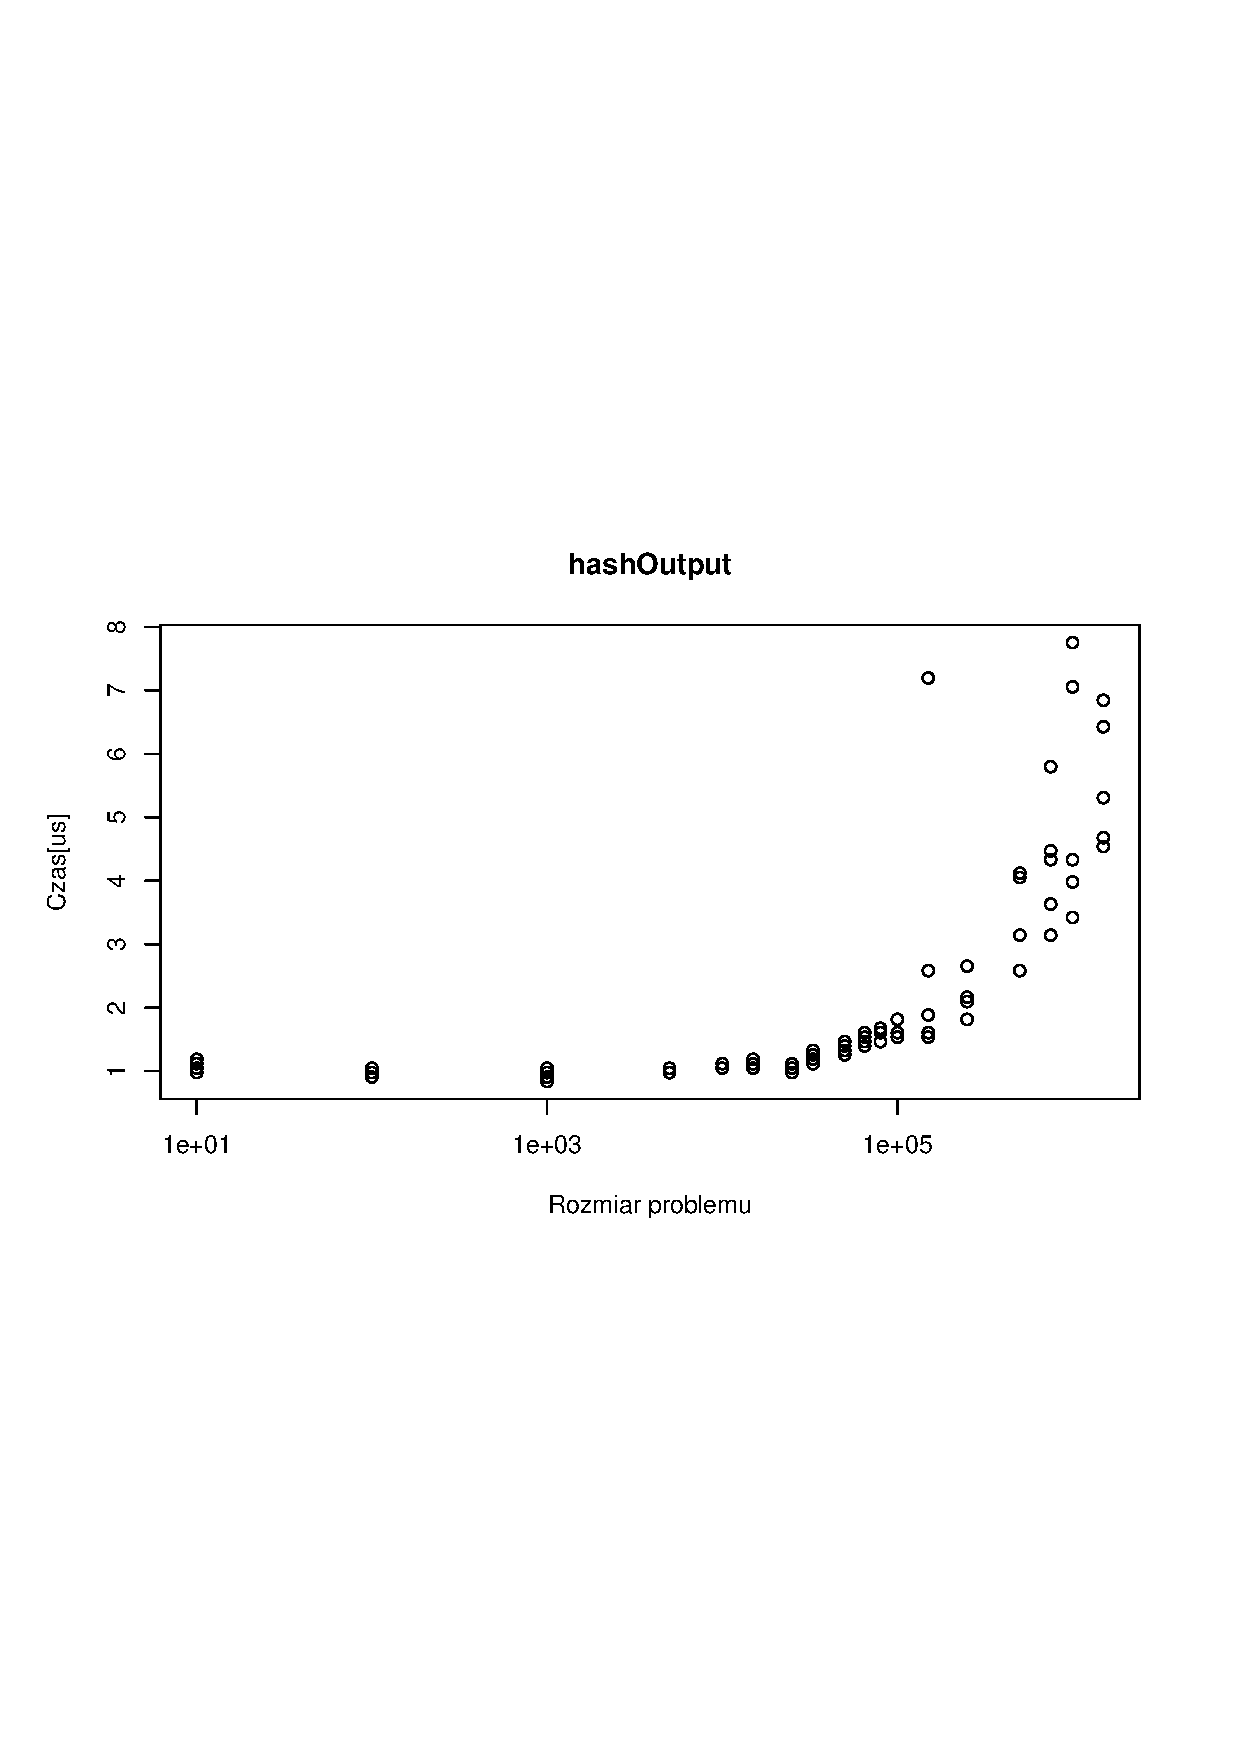
\includegraphics[width=0.7\linewidth]{./Wykresy/hashOutput}
\caption{Wyniki dla tablicy mieszającej}
\label{fig:hashOutput}
\end{figure}

\begin{figure}[H]
\centering
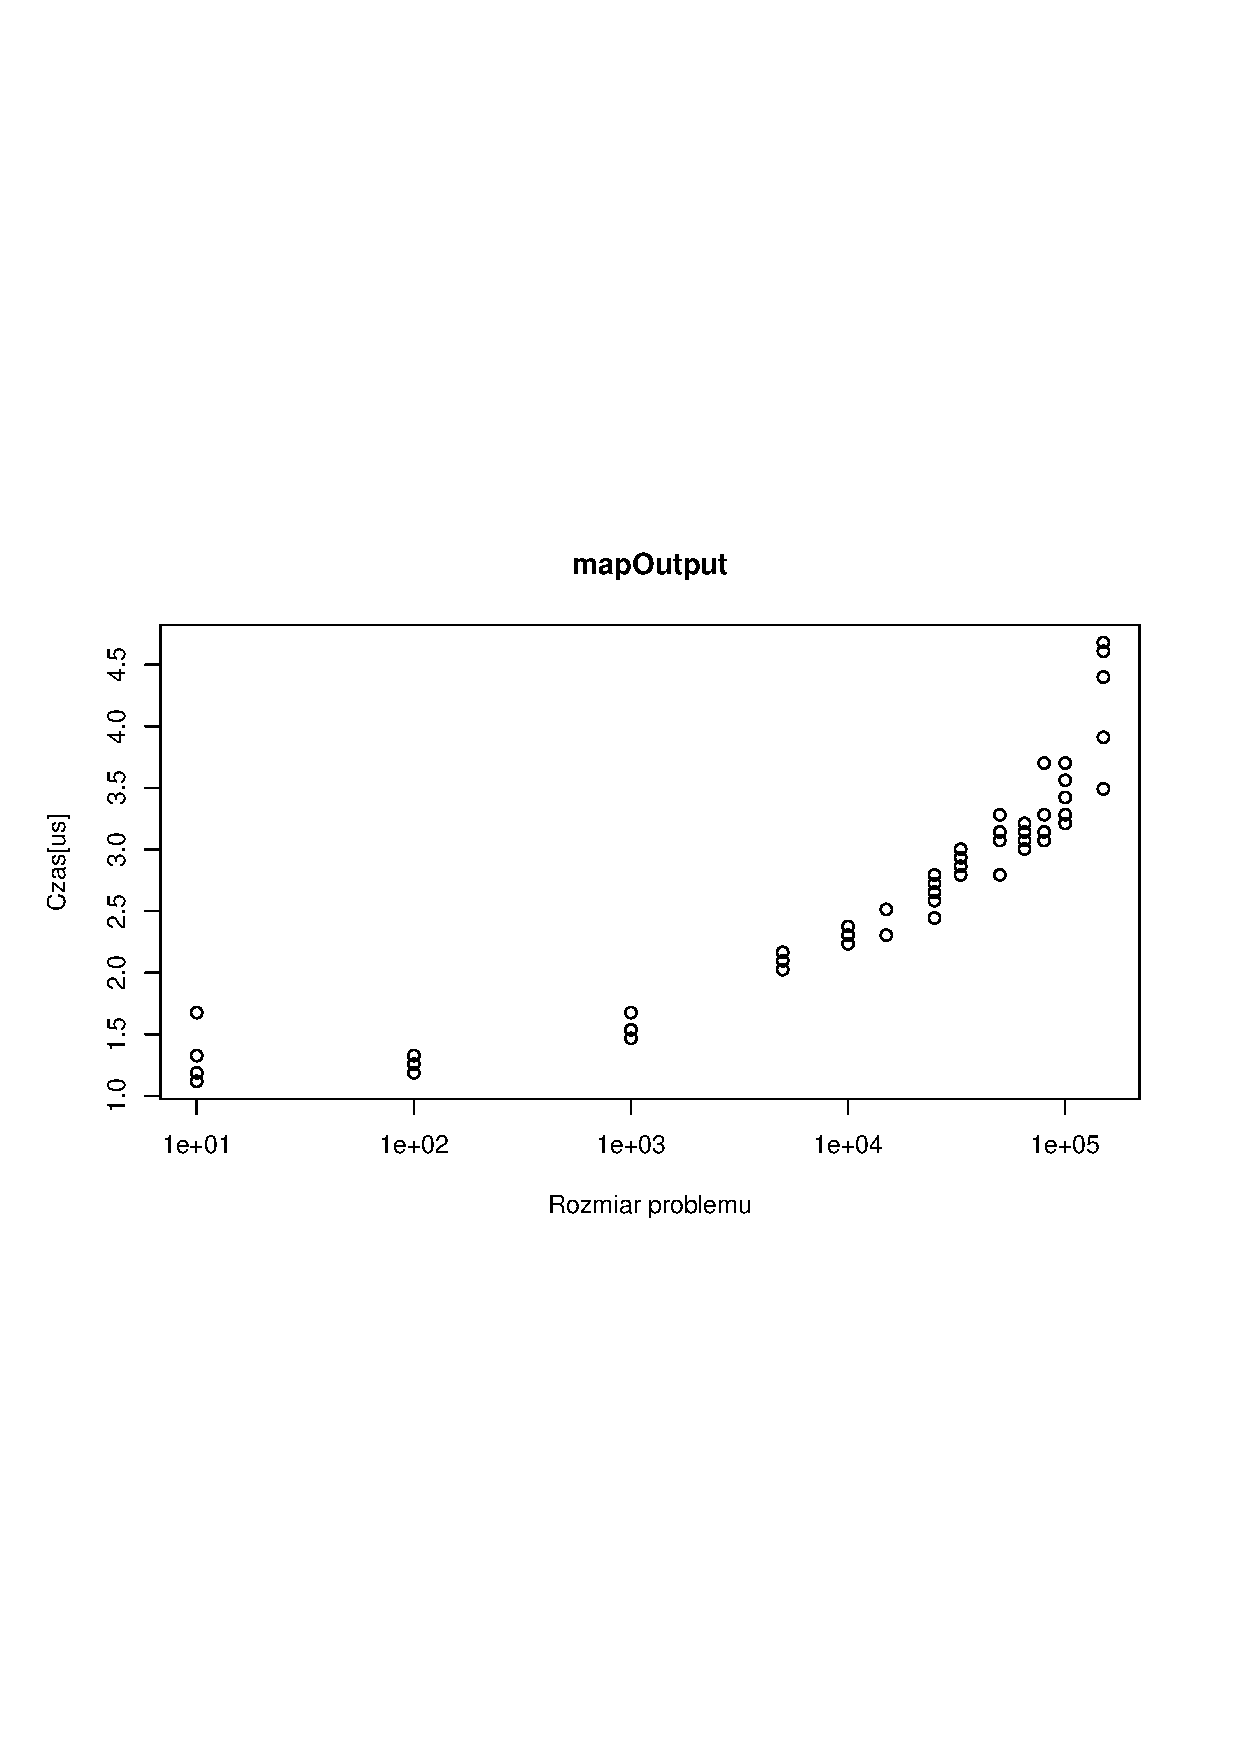
\includegraphics[width=0.7\linewidth]{./Wykresy/mapOutput}
\caption{Wyniki dla tablicy asocjacyjnej zbudowanej na \textit{std::vector}}
\label{fig:mapOutput}
\end{figure}



\section{Wnioski oraz uwagi}

Na podstawie przeprowadzonych testów można wysnuć następujące wnioski:
\begin{itemize}
\item Widać, że czas dostępu nie zależy tylko od rozmiaru problemu, sposób uporządkowania
danych oraz ich różnorodność jest również istotna, stąd duże rozbieżności w czasie dostępu
do elementu dla takiego samego rozmiaru danych.
\item Tablica mieszająca, dla dużego rozmiaru ma gorszy czas od drzewa przeszukiwań binarnych,
ponieważ występują kolizje i należy dodatkowo szukać w listach w czasie liniowym
\item Implementacja na \textit{std::vector} i na drzewie przeszukiwań, co można
w przybliżeniu zaobserwować na wykresach, ma czas ~$\mathcal{O}(log(n)$,
tablica mieszająca ma problemy dla liczniejszych zbiorów, występują kolizje, jest to złożoność
$\mathcal{O}(nlog(n))$
\item Implementacja na \textit{std::vector} nie nadaje się do przechowywania bardzo dużej ilości
danych, ponieważ złożoność dodania elementu do tablicy jest liniowa
\end{itemize}

\end{document}